\documentclass{article}
\usepackage[utf8]{inputenc}
\usepackage{graphicx,booktabs,subcaption,amsmath,wrapfig,float}
\usepackage[super,sort&compress]{natbib} % citas numéricas en superíndice
\usepackage[hidelinks]{hyperref}         % \href y enlaces; cargar el último
\graphicspath{{images/}}
\renewcommand{\refname}{Referencias}
\setlength{\bibsep}{1pt}
\setlength{\textfloatsep}{10pt plus 2pt minus 2pt}
\begin{document}
\section{Datos del proyecto}
\begin{itemize}
    \item \textbf{Código de grupo:} 
    \item \textbf{Participantes:} Nicolás Mínguez Aguirre
    \item \textbf{Título:} Efecto de \textit{El Niño Southern Oscillation (ENSO)} en \textit{Snow Water Equivalent (SWE)} según zonas y elevaciones del \textit{Pacific Northwest, EE.UU.}
    \item \textbf{Enlace dataset:}
\end{itemize}
\section{Presentación}
En la zona del \textit{Pacific Northwest} en la costa oeste del pacífico, la cantidad de agua acumulada en la nieve, medida en \textit{Snow Water Equivalent} (SWE) es útil para anticipar sequías o inundaciones. Esta variable depende de muchos factores: desde temperatura y precipitación, hasta circulaciones atmosféricas, humedad, radiación solar y muchos otros inmedibles. 
Sin embargo, el índice de anomalía de la temperatura superficial del mar en la región Niño 3.4 (ENSO)\cite{psl} resume en un solo indicador el estado de la circulación atmosférico-oceánica de gran escala que condiciona esos factores. Por ello, aunque no sea el mejor predictor de SWE, es especialmente útil, porque sus oscilaciones permiten predicciones con más antelación que otros factores, y es externo al SWE (el SWE no influye en el ENSO).
La cuestión de interes es si la señal de ENSO en el SWE difiere según zona o elevación dentro de la región.
\begin{center}
ENSO $\rightarrow$ \{TAVG, PRCP, otros factores\} $\xrightarrow[\text{elevación}]{\text{zona}}$ SWE
\end{center}
\section{Dataset}
\textit{Dataset} construido a partir de dos fuentes:
\begin{itemize}
    \item \textbf{SNOTEL}: red automática de sensores de nieve y clima de montaña del NRCS (USDA) en el oeste de EE.UU.; datos mensuales y metadatos de estación vía API REST AWDB\cite{awdb}.
\item \textbf{NOAA PSL}: laboratorio de la NOAA de investigación meteorológica, climática e hidrológica; anomalía mensual de temperatura superficial del mar en Niño 3.4 (ENSO) vía .csv\cite{psl}.
\end{itemize}
La mayor parte de SNOTEL se instaló alrededor del 1980\cite{mote2008}, lo que fija el estudio en los inviernos 1980/81-2025/26; cada invierno se denota por el año en que termina (2025/26 $\rightarrow$ temporada 2026).
\begin{table}
\centering
\small
\begin{tabular}{llp{5.6cm}}
\toprule
Fuente & Tipo & Variables \\
\midrule
SNOTEL & Categórica nominal & \texttt{station\_id}, \texttt{station\_name}, \texttt{huc6}$^{*}$, \texttt{zone\_name}\\
SNOTEL & Numérica discreta & \texttt{season*}\\
SNOTEL & Numérica & \texttt{TAVG}, \texttt{PRCP}, \texttt{SWE}$^{*}$, \texttt{latitude}, \texttt{longitude}, \texttt{elevation\_m}$^{*}$ \\
NOAA PSL & Numérica & \texttt{ENSO}$^{*}$\\
\bottomrule
\end{tabular}
\caption{Variables del dataset. $^{*}$Usadas en el estudio.}
\label{tab:dataset}
\end{table}
 \newpage
 \section{Objetivos}
El trabajo recoge los datos dentro de la zona y franja temporal de estudio definidos, luego se estudian y se preparan esos datos, y finalmente se aplica un breve ANOVA para ver si el modelo resulta significativo.
\begin{center}
\small Fuentes $\xrightarrow[\text{recolección}]{\text{O1}}$ DS1 $\xrightarrow[\text{preparación}]{\text{O2}}$ DS2 $\xrightarrow[\text{análisis}]{\text{O3}}$ DS3 (ANOVA)
\end{center}
 \subsection{O1: Qué puntos existen?}
 \begin{itemize}
 \item Decidir la unidad temporal del estudio considerando la granularidad de las variables y resolver la autocorrelación temporal de SWE y ENSO. 
 \item Decidir como agregar SWE, ENSO, PRCP, TAVG, y si es adecuado codificar la zona o elevacion.
 \end{itemize}
 \subsection{O2: Qué puntos sirven?}
 \begin{itemize}
     \item Tratar puntos con mediciones incompletas en SWE y ENSO y considerar si la eliminación de una instancia resulta en datos sesgados.
     \item Decidir cantidad y dispersión necesarias para los puntos de cada estación.
\end{itemize}
 \subsection{O3: Como usamos los puntos?}
 \begin{itemize}
\item Decidir si SWE y ENSO requieren transformación para que la pendiente sea comparable entre estaciones.
\item Estudiar la asociación entre zona y elevación y si es neceasrio restringir las estaciones a un rango de elevación común.
\item Analizar la señal $\beta_1$ según zona y elevación mediante un ANOVA parsimonioso e interpretar resultados.
 \end{itemize}
\section{Desarrollo}
\subsection{O1: Qué puntos existen?}
\subsubsection{Unidad temporal}
Los datos de cada estación son mensuales, pero usar el mes como unidad produce observaciones fuertemente correladas (Fig.~\ref{fig:swe_enso_station}): tanto el SWE como el ENSO dependen del mes anterior. Se condensan en temporadas (dic--abr) para separar temporalmente las observaciones. En las estaciones estudiadas la nieve se funde por completo, por lo que se espera incorrelación del SWE entre temporadas, mientras que se espera que el nivel de autocorrelación de ENSO disminuya.
\begin{figure}[htbp]
  \centering
  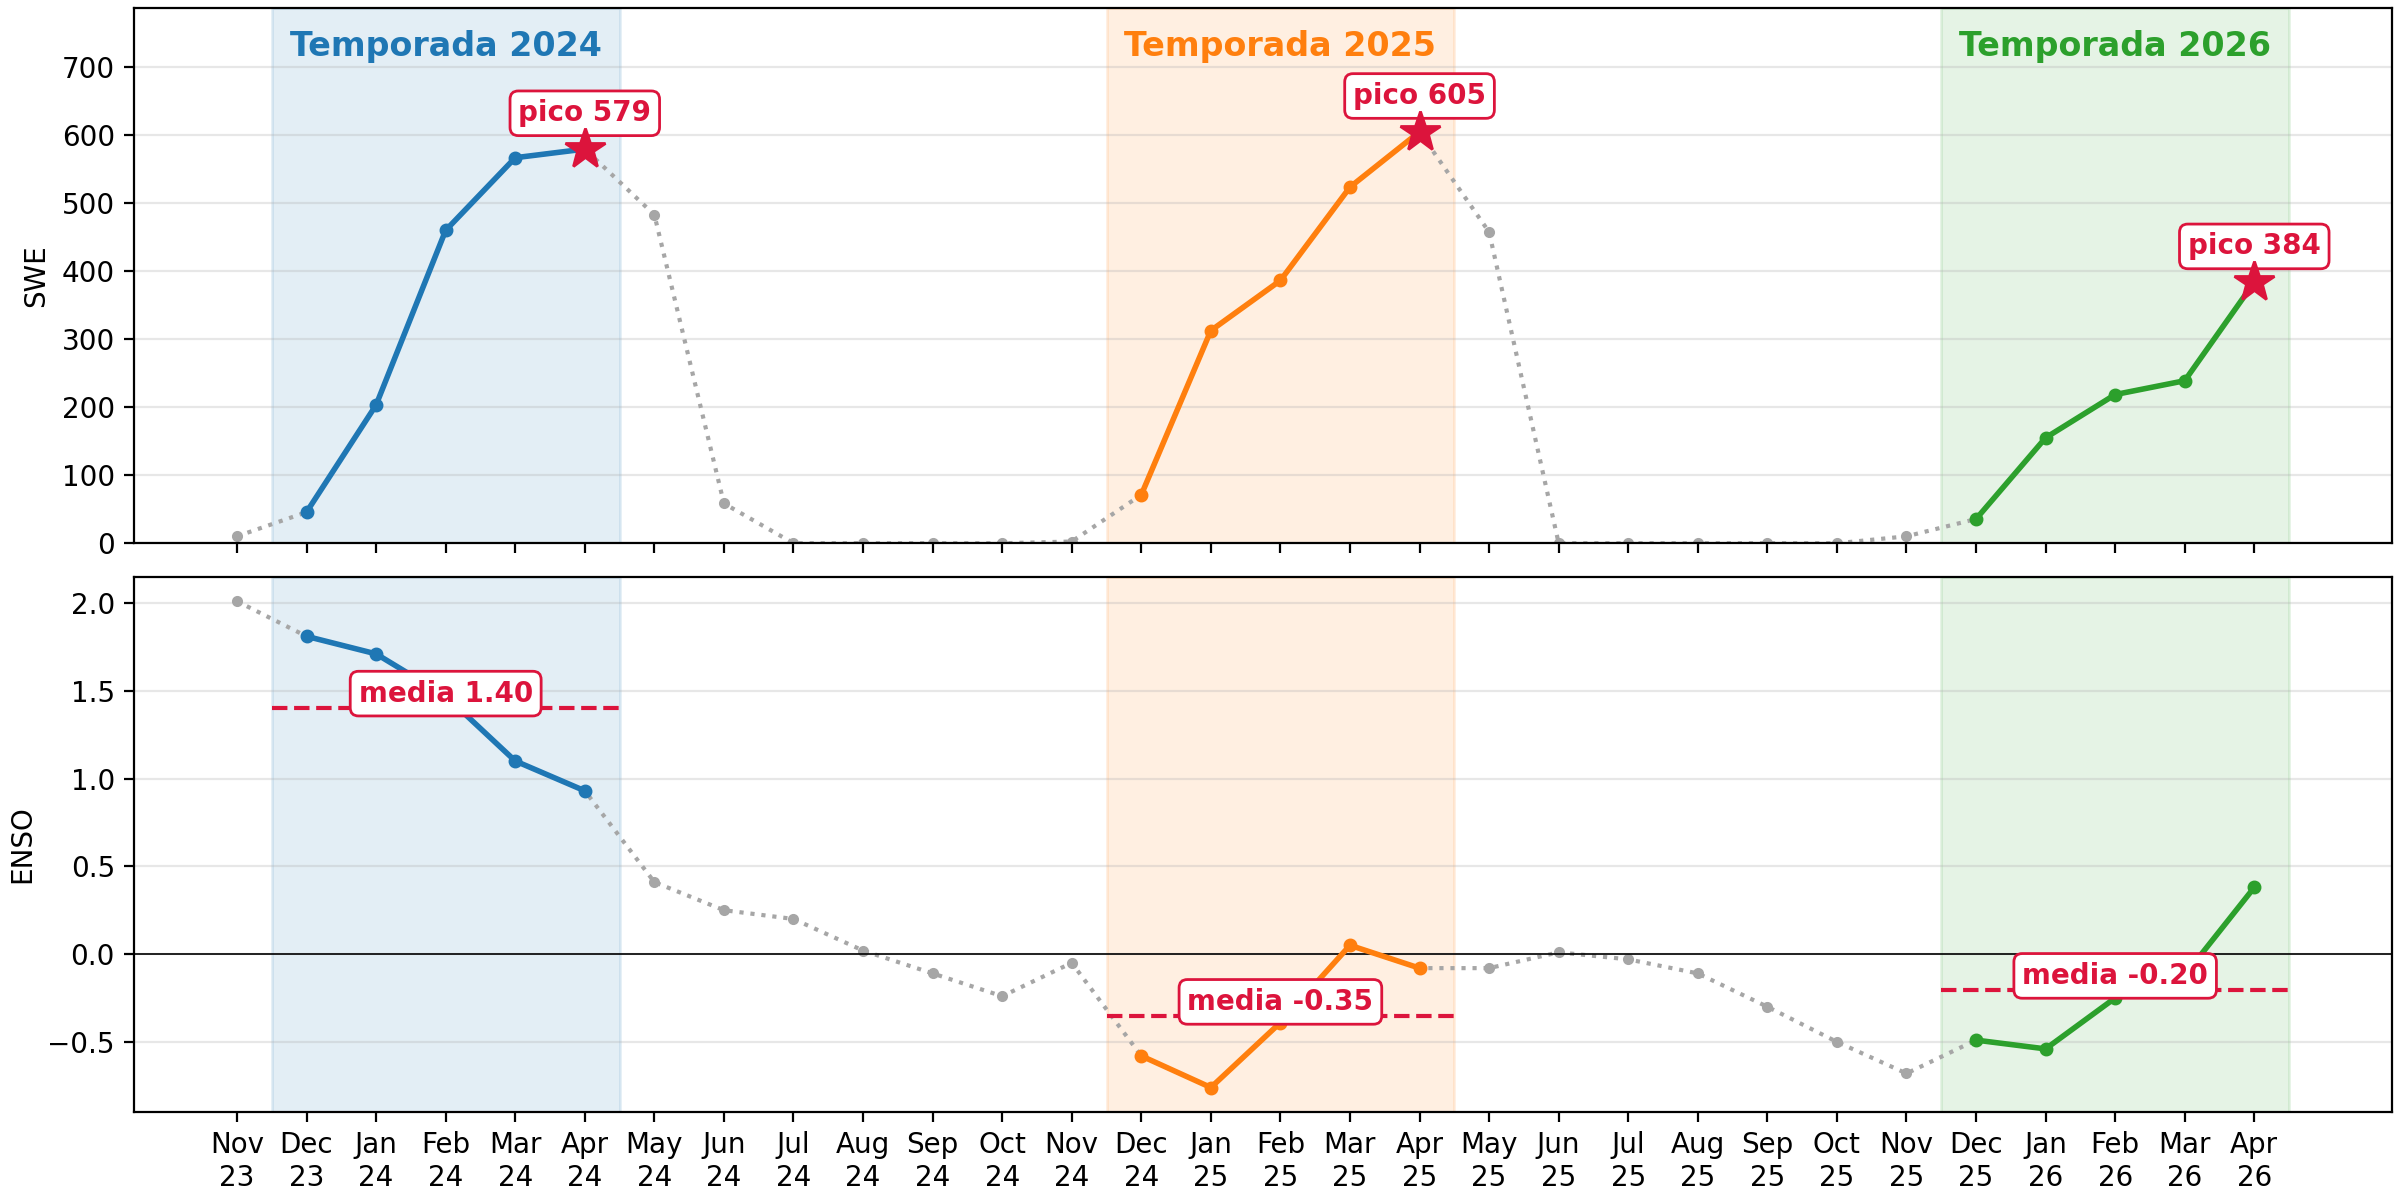
\includegraphics[width=\linewidth]{o1/swe_enso_station.png}
  \caption{SWE mensual y anomalía de Niño 3.4 (ENSO) en 2023-2026 en \textit{Stampede Pass}, estación meteorológica representativa de la región\cite{mote2008}.}
  \label{fig:swe_enso_station}
\end{figure}
\begin{table}[ht]
\centering
\small
\setlength{\tabcolsep}{3pt}
\begin{subtable}[b]{0.42\linewidth}
\centering
\begin{tabular}{lrr}
\toprule
Mensual & 1 mes & 12 meses \\
\midrule
SWE bruto    & 0.81 & 0.76 \\
SWE anomalía & 0.80 & 0.10 \\
ENSO$^{*}$   & 0.95 & $-$0.07 \\
\bottomrule
\end{tabular}
\caption{Antes (mensual)}
\end{subtable}
\hfill
\begin{subtable}[b]{0.54\linewidth}
\centering
\begin{tabular}{lrrr}
\toprule
Estacional & 1 temp.& 2 temp.& 3 temp.\\
\midrule
SWE (\textit{peak})  & 0.08    & 0.23    & $-$0.08 \\
ENSO (\textit{mean}) & $-$0.04 & $-$0.37 & $-$0.04 \\
\bottomrule
\end{tabular}
\caption{Después (anual)}
\end{subtable}
\caption{$^{*}$Niño 3.4 ya es una anomalía.}
\label{tab:ac}
\end{table}

La tabla (Tab.~\ref{tab:ac}) muestra la autocorrelación muestral ($r_{\mathrm{Pearson}}$) en \textit{Stampede Pass}. La serie mensual incluye la anomalía de SWE (sin la media de cada mes, para excluir el ciclo estacional); la estacional usa el pico de SWE y la media del ENSO. $^{*}$Niño 3.4 ya es una anomalía.

A nivel mensual la dependencia es fuerte (anomalía de SWE 0.80, ENSO 0.95): el tamaño efectivo se reduce a $n_{\mathrm{ef}}\approx5$ para el SWE y $n_{\mathrm{ef}}\approx1$ para el ENSO, e inflaría la significación. Tras condensar por temporada la dependencia disminuye (SWE 0.08, ENSO $-$0.04) y $n_{\mathrm{ef}}$ es del orden de $n$. La excepción es el ENSO a dos temporadas ($-0.37$), que supera la banda $\pm2/\sqrt{n}\approx\pm0.3$ y refleja la alternancia habitual de fases\cite{psl}; se asume como dependencia residual.

\subsubsection{Agregación}
La unidad de instancia es la temporada, y una muestra independiente, una estación-temporada. Las variables numéricas, funciones del mes dentro de cada temporada, se agregan como indica la Tabla~\ref{tab:agg}.
\begin{table}[ht]
\centering
\small
\renewcommand{\arraystretch}{1.25}
\begin{tabular}{llp{7.8cm}}
\toprule
Variable (funcional)& Agregación & Razón  \\
\midrule
SWE (mm)& máximo & Mide mayor volumen acumulado, que no necesariamente ocurre en una fecha fija.\\
TAVG (Celsius)& media  & Resume la persistencia sin explotar ruido mensual.\\
PRCP (mm)& suma   & Mide volumen acumulado de forma análoga al SWE.\\
ENSO (Celsius)& media  & Resume la persistencia sin explotar ruido mensual.\\
\bottomrule
\end{tabular}
\label{tab:agg}
\end{table}

\begin{wrapfigure}{r}{0.3\textwidth}
\centering
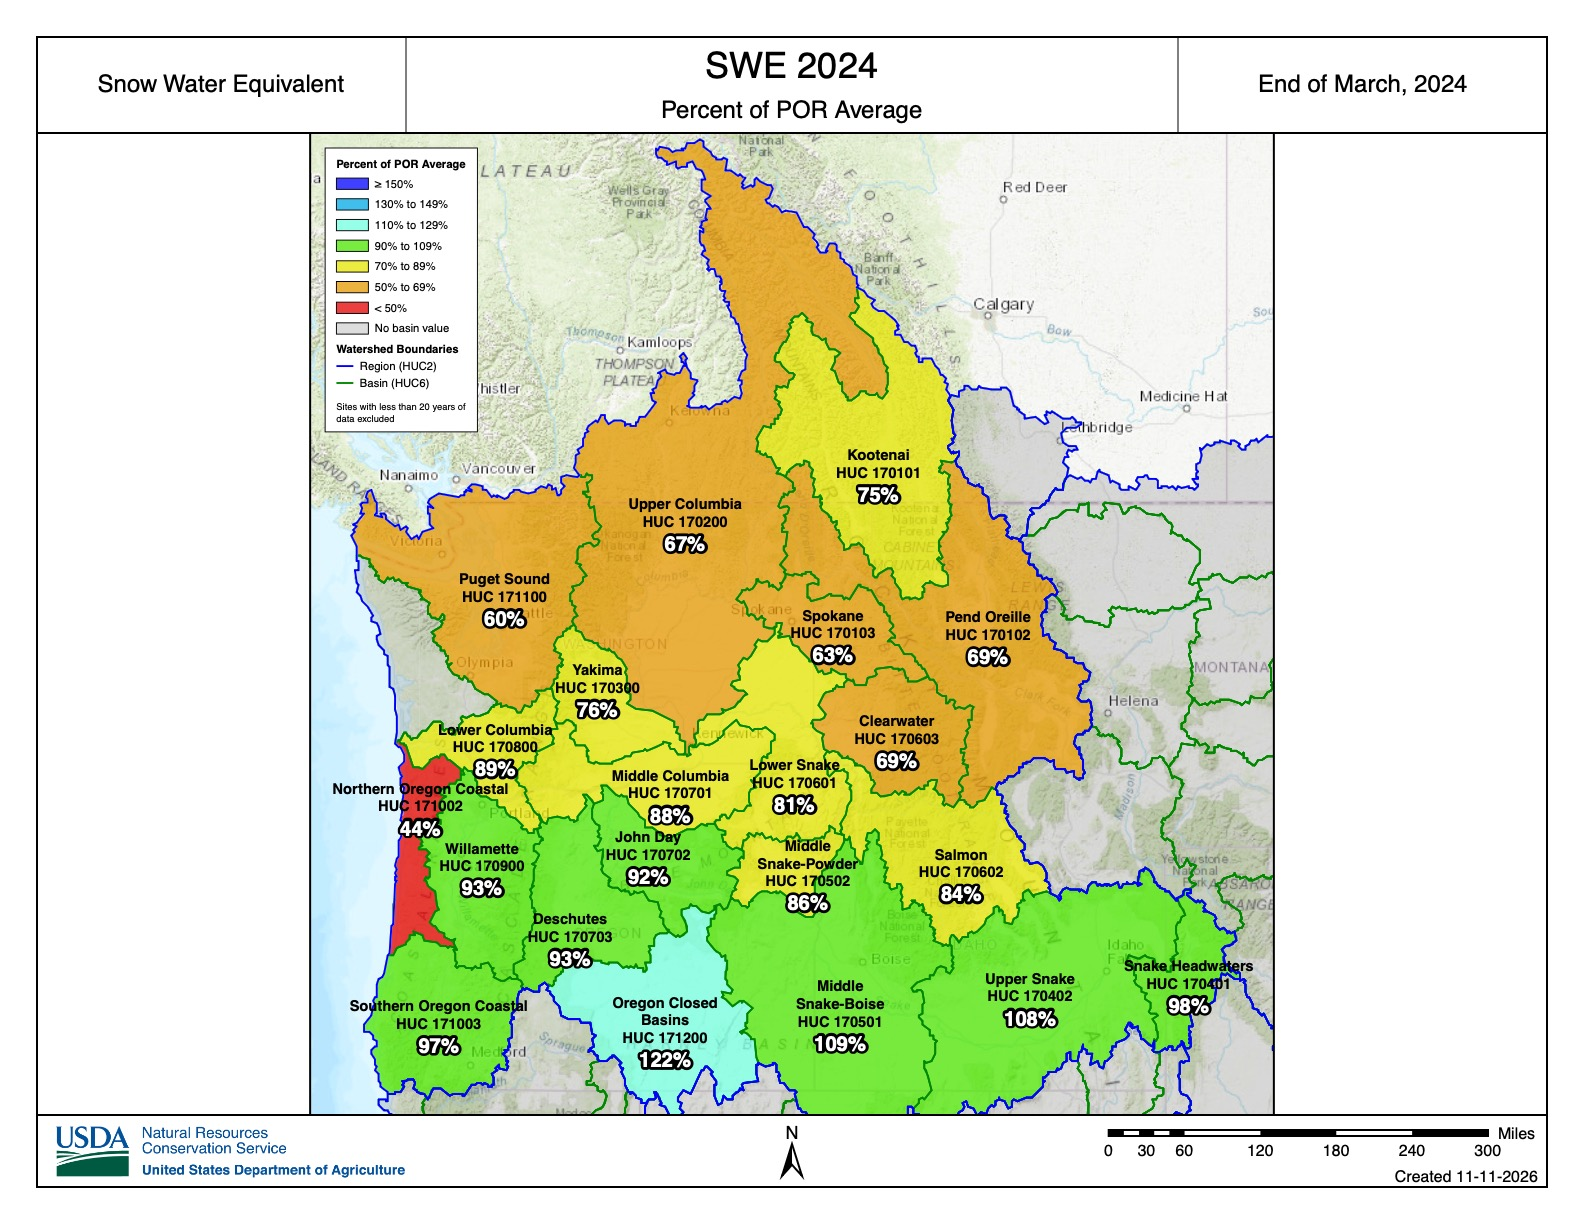
\includegraphics[width=\linewidth]{usda/swe_2024_map.jpeg}
\caption{Mapa de SWE en 2024 (USDA)\cite{imap}.}
\label{fig:map}
\end{wrapfigure}
TAVG y PRCP no entran al modelo; se conservan en DS1 para la detección de valores atípicos. Zona (Fig.~\ref{fig:map}) y elevación son constantes en cada estación y se conservan sin codificar: la elevación es continua y exacta, y la zona es una etiqueta nominal, pues cualquier condificación numérica derivada de la geografía (coordenadas, distancia a la costa o a un centroide) incorporaría la elevación mediante la superficie terrestre, y el código HUC solo refleja jerarquía administrativa. Su relación se estudia en O3.

\subsection{O2: Qué puntos sirven?}
\subsubsection{Mediciones incompletas}
Solo SWE y ENSO entran al modelo; para ellos, la incompletud de una estación-temporada implica:
\begin{itemize}
\item SWE (máximo): si falta un mes (p.~ej., marzo), probablemente no se mide el pico real y el valor se subestima, por lo que no es comparable con el de una temporada completa.
\item ENSO (media): no tiene valores faltantes; no requiere tratamiento.
\end{itemize}
Se eliminan las estación-temporadas sin los cinco meses de la ventana dic--abr ($3.30\%$) en lugar de imputar el SWE. Imputarlo con estaciones vecinas (\textit{hot-deck} por vecinos más cercanos) incorpora por construcción la señal de ENSO que comparten (\textit{data leakage}), y con otras temporadas de la misma estación (p.~ej., su media) atenúa la pendiente; en ambos casos se añaden filas sin información independiente. La eliminación solo sesgaría la pendiente si la ausencia dependiera del ENSO (p.~ej., fallos de sensores en tormentas intensas); se contrasta con la correlación de Spearman entre el ENSO de cada temporada y la fracción de estaciones descartadas en ella ($\rho=0.1105$, $p=0.4646$).

\subsubsection{Cantidad y dispersión de puntos por estación}
Se examina \textit{Stampede Pass}, con densidad temporal consistente (Fig.~\ref{fig:enso_swe}).
\begin{figure}[htbp]
\centering
\begin{subfigure}{.48\linewidth}\centering
\caption{Temporada y SWE en \textit{Stampede Pass}}
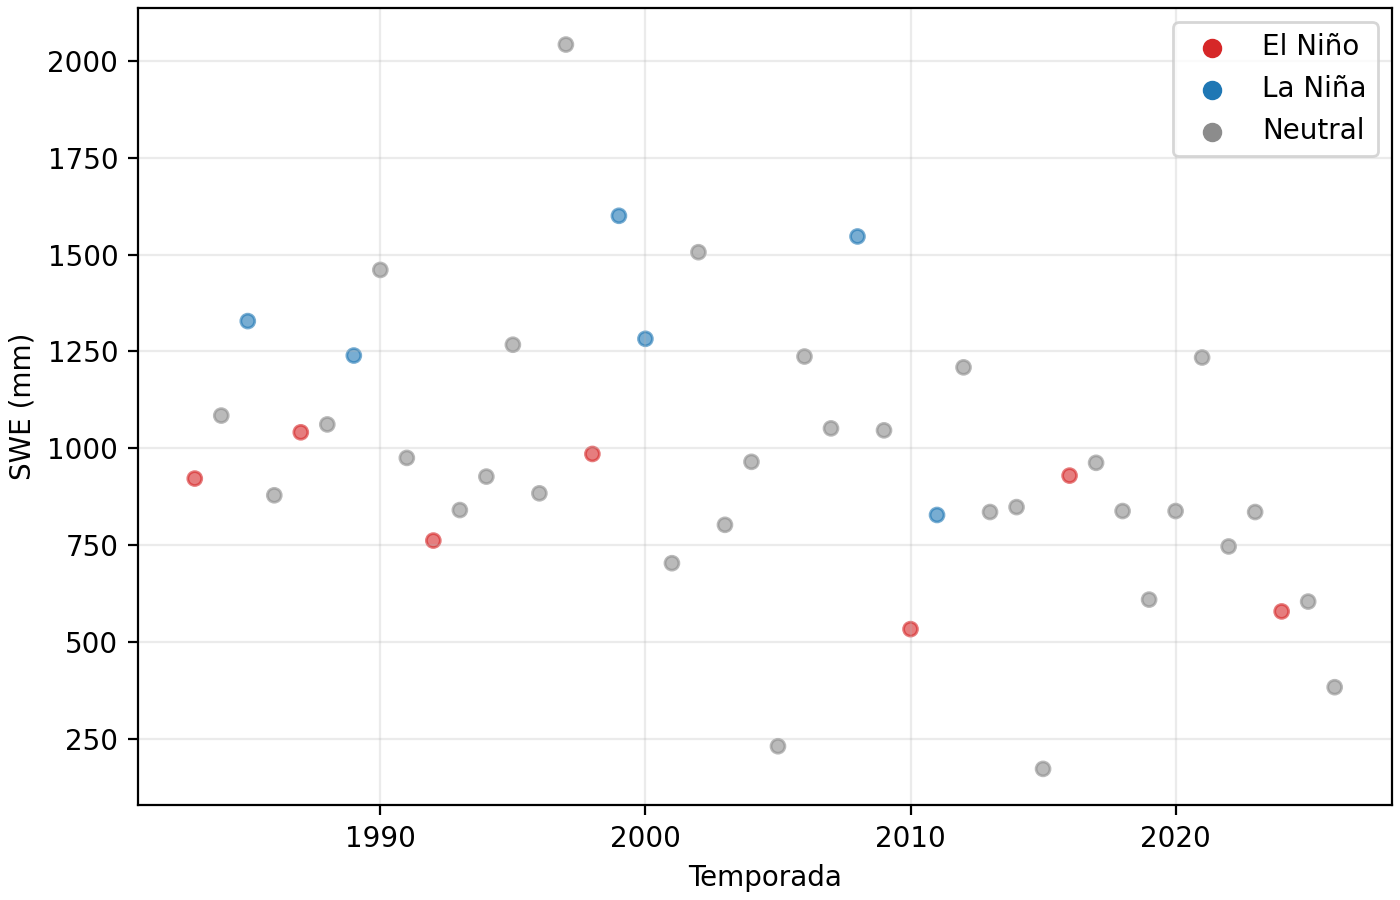
\includegraphics[width=\linewidth]{o2/year_enso_vs_swe.png}
\end{subfigure}
\hfill
\begin{subfigure}{.48\linewidth}\centering
\caption{ENSO y SWE en \textit{Stampede Pass}}
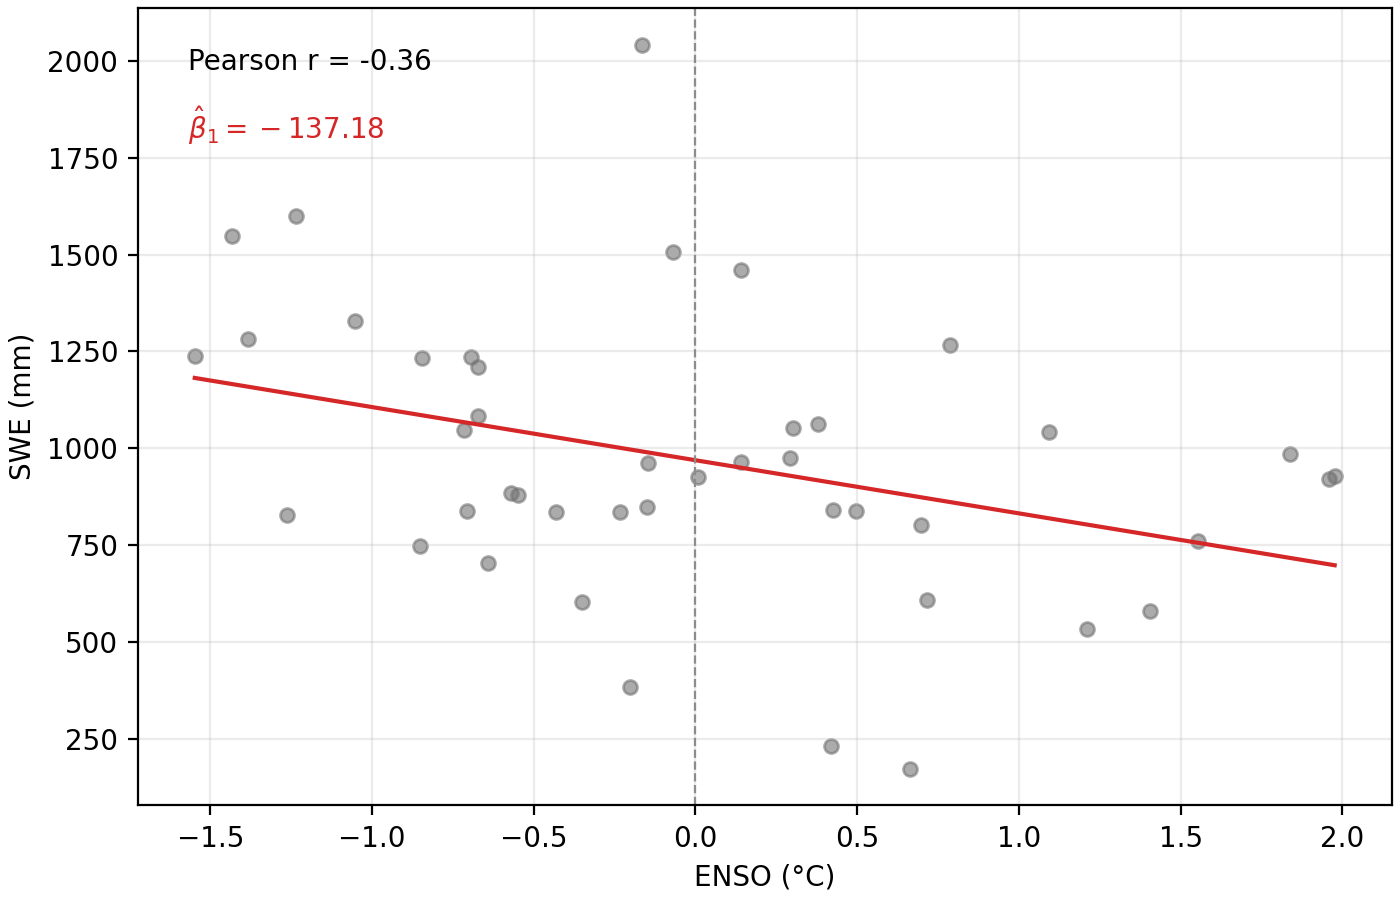
\includegraphics[width=\linewidth]{o2/enso_vs_swe.png}
\end{subfigure}
\caption{Señal SWE$\sim$ENSO en \textit{Stampede Pass}.}
\label{fig:enso_swe}
\end{figure}
Se observan dos patrones:
\begin{itemize}
\item El SWE tiende a ser mayor en La Niña que en El Niño, con variabilidad considerable (algunas temporadas Niño superan a algunas Niña): la señal existe pero es moderada.
\item El SWE decrece con el tiempo, sobre todo en los últimos años, por factores ajenos al ENSO (circulación atmosférica, calentamiento a largo plazo): se controla en O3 para no atribuirlo al ENSO.
\end{itemize}
Ajustar una recta en (b) es razonable, pero su pendiente solo se estima con precisión si la estación tiene suficientes temporadas y sin grandes huecos en los extremos. Se impone un único límite que cubre ambos: $m\ge30$ de las 46 temporadas (como mucho 15 sin medición), con lo que el \textit{dataset} pasa de $X=11085$ a $Y=10021$ estación-temporadas. 
\subsection{O3: Cómo usamos los puntos?}

Interesa saber si la pendiente en (Fig.~\ref{fig:enso_swe}) cambia con la zona y la elevación. Para compararla entre estaciones hay que fijar la escala de SWE y ENSO y asegurar que zona y elevación no se confunden.

\subsubsection{SWE y ENSO}
Las unidades no afectan al contraste, pero la escala sí: en mm, el efecto absoluto del ENSO crece con el volumen de nieve, y por tanto con la elevación, aun con el mismo efecto relativo; comparar $\beta_1$ en bruto mezclaría ambos. Por ello se usa $\log(1+\mathrm{SWE})$ (Box--Cox con $\lambda=0$ y desplazamiento 1 por los valores nulos; $\hat\lambda=0$), con lo que $\beta_1$ es un efecto multiplicativo comparable entre estaciones y la asimetría cambia de $1.2365$ a $-1.7669$ (Fig.~\ref{fig:dist}). El ENSO ya es una anomalía aproximadamente simétrica (asimetría $0.4533$), aunque no se fuerza normalidad; solo se estandariza a $\sigma$ para expresar $\beta_1$ por desviación típica, sin cambiar su forma (Fig.~\ref{fig:dist}). No se estandariza el SWE por estación: dividir por una desviación propia de cada estación impediría leer $\beta_1$ como multiplicador.
\begin{figure}[htbp]
\centering
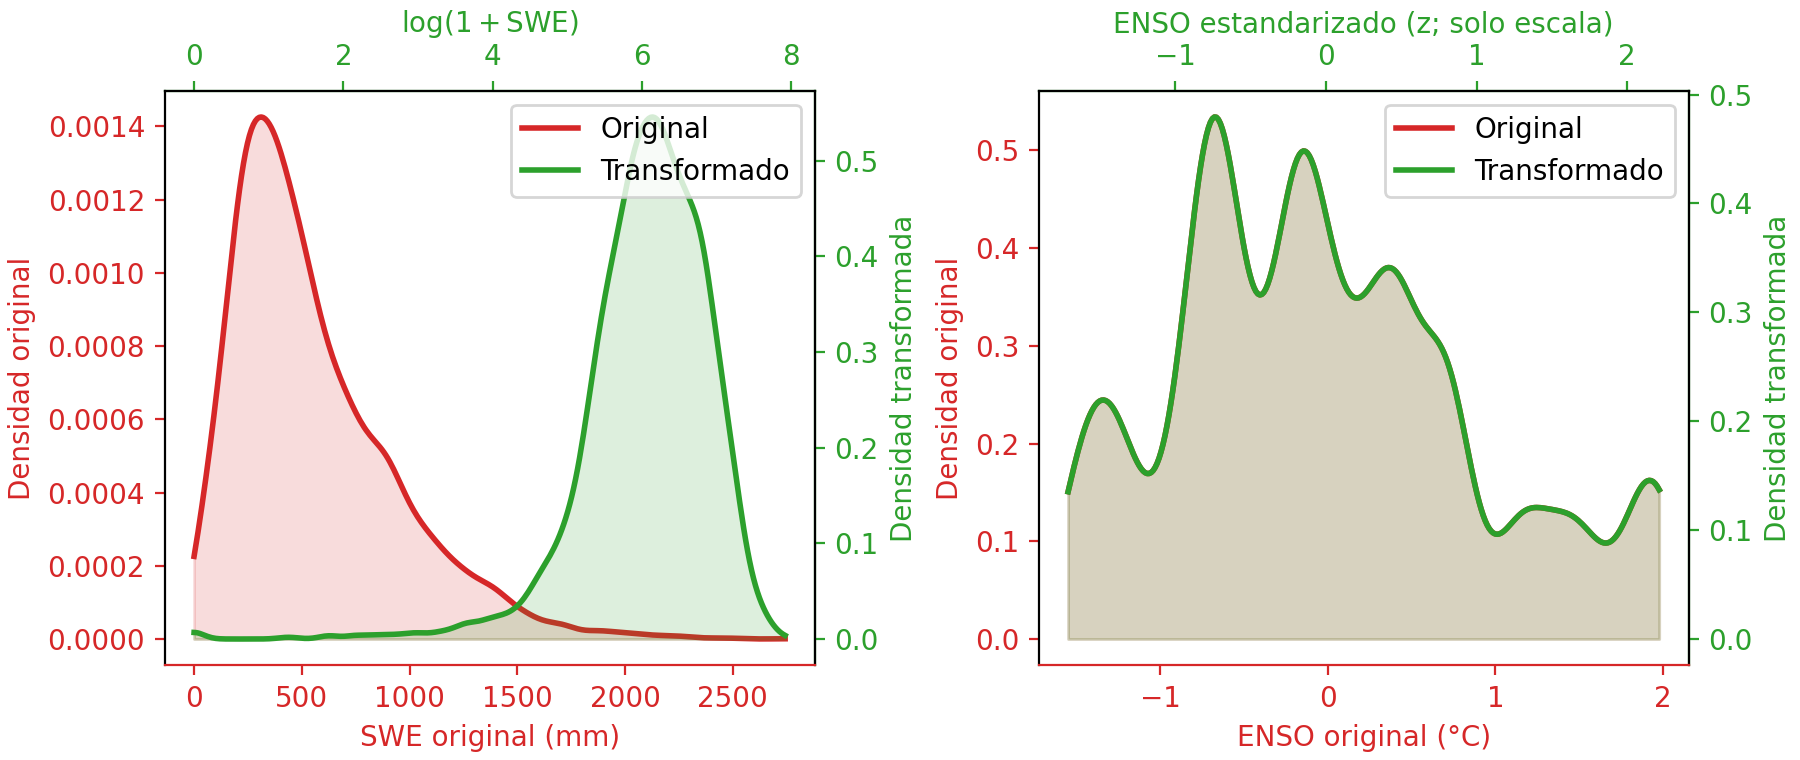
\includegraphics[width=.9\linewidth]{o3/distributions.png}
\caption{Densidades de SWE y ENSO antes y después de la transformación, con ejes independientes (rojo: unidades originales, verde: unidades transformadas). El modelo usa $\log(1+\mathrm{SWE})$ sin estandarizar por estación y ENSO estandarizado globalmente; esta estandarización cambia la escala, pero no normaliza ENSO.}
\label{fig:dist}
\end{figure}

\subsubsection{Zona y elevación}
Las zonas ocupan rangos de elevación distintos, así que $\beta_1$ frente a la zona arrastraría la elevación, y viceversa. Se ilustran tres estaciones representativas, a elevaciones baja, media y alta, según su zona (HUC6 como proxy) y elevación (Fig.~\ref{fig:o3}a). Se fija una banda de elevación $[630.9,2816.4]\,\mathrm{m}$ en la que toda zona conservada tenga al menos 3 estaciones; se descartan las estaciones fuera de la banda y las zonas que no llegan a 3 (0 zonas). La banda se fija sin usar SWE ni $\beta_1$, para no sesgar la selección. La confusión se mide con la $\eta^2$ ajustada de la elevación por zona ($R^2$ de elevación$\sim$zona), preferible a la $V$ de Cramér, que exigiría discretizar la elevación; el valor es $0.6479$ antes y después, por lo que ambas variables no son completamente separables. Tras la restricción, la relación de $\beta_1$ por estación (de $\log(1+\mathrm{SWE})\sim\mathrm{ENSO}+\mathrm{temporada}$) con la elevación se ilustra con tres estaciones (Fig.~\ref{fig:o3}b); el ajuste cuadrático con todas las estaciones es cóncavo ($p=2.405\times10^{-26}$): se espera un $|\beta_1|$ máximo en torno al umbral lluvia--nieve ($\beta_1<0$), una campana que un término lineal no capta.
\begin{figure}[H]
\centering
\begin{subfigure}[t]{.48\linewidth}\centering
\caption{Tres estaciones representativas y banda común}
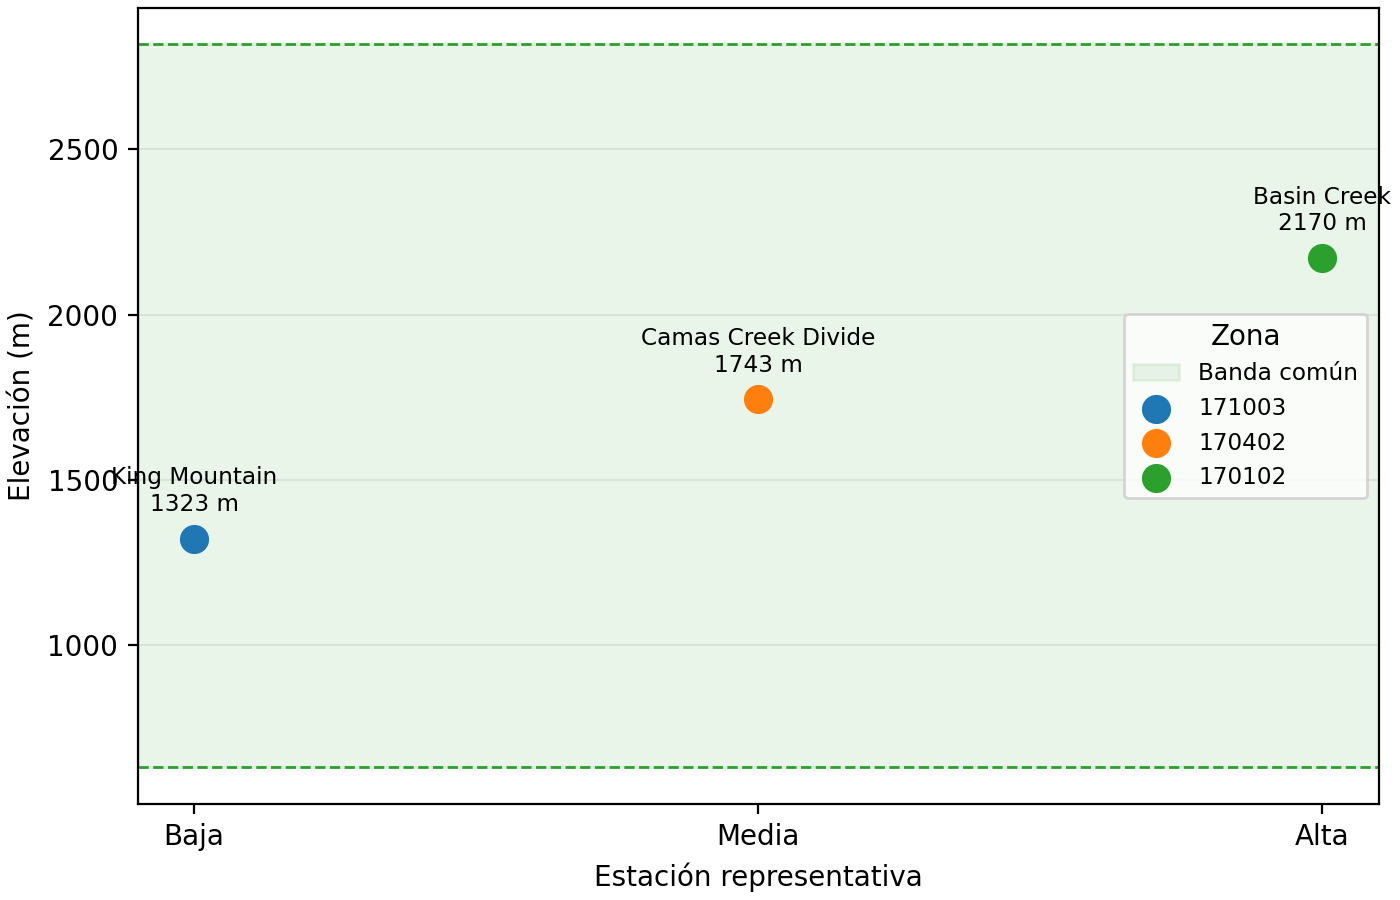
\includegraphics[width=\linewidth]{o3/stations_zone_elevation.png}
\end{subfigure}
\hfill
\begin{subfigure}[t]{.48\linewidth}\centering
\caption{$\hat{\beta}_1$ por elevación en tres estaciones}
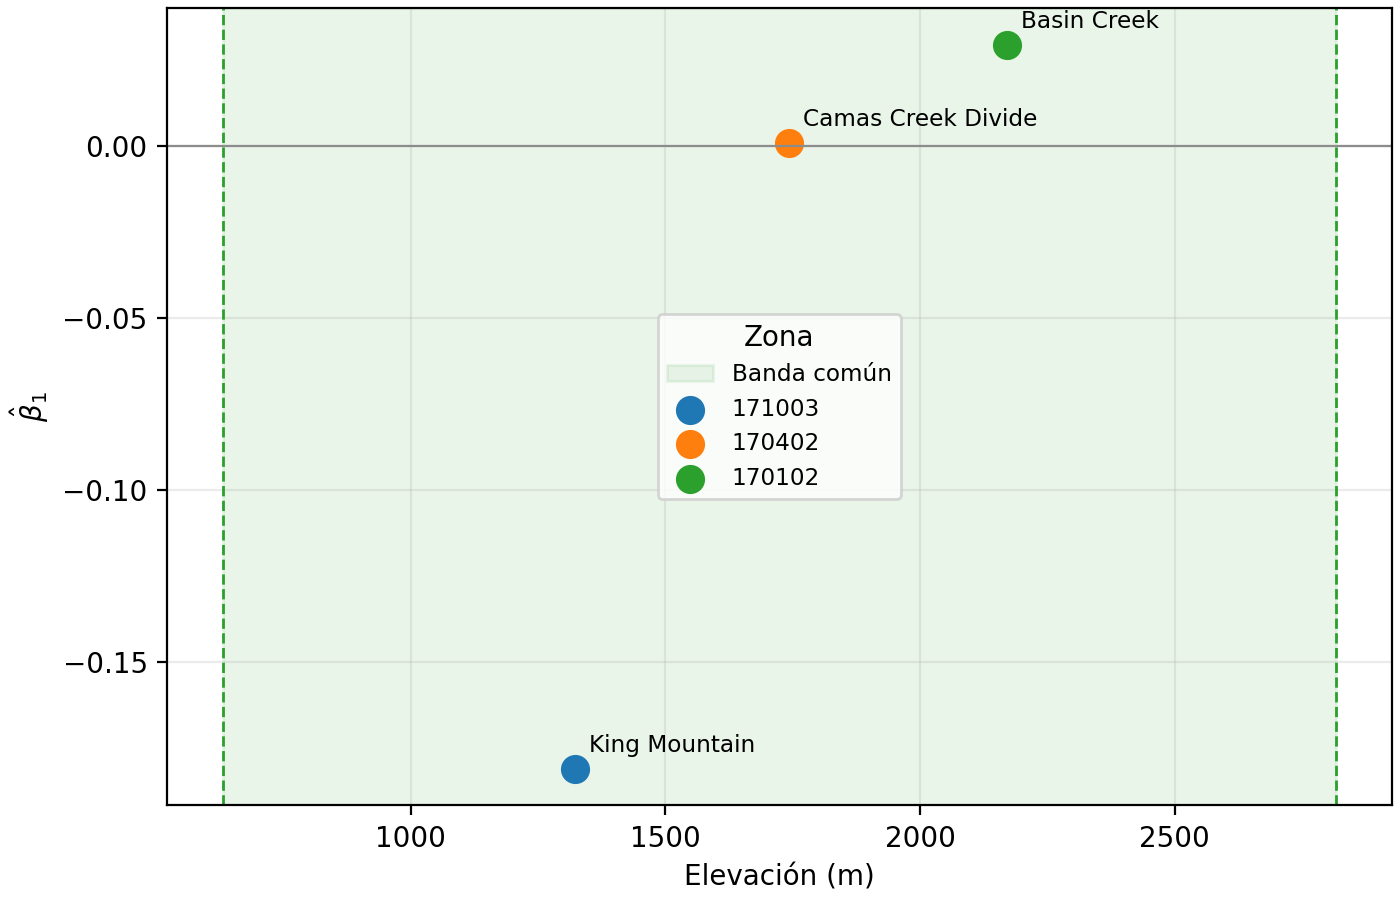
\includegraphics[width=\linewidth]{o3/beta_elevation.png}
\end{subfigure}
\caption{Zona y elevación: (a) tres estaciones representativas y banda común; (b) pendiente por estación.}
\label{fig:o3}
\end{figure}
\subsubsection{Modelo} Se ajusta \texttt{log1p(SWE) $\sim$ temporada + zona + elev + ENSO + ENSO:zona + ENSO:elev} con sumas de cuadrados tipo II: las dos interacciones responden a la pregunta del estudio, y se omiten la triple y zona:elev por parsimonia. La zona es nominal; la elevación se factoriza en terciles dentro de la banda, pues una campana no cabe en un término lineal y los terciles la captan sin imponer forma (se pierde información intra-tercil; el \textit{dataset} conserva \texttt{elevation\_m}; se observan 18 celdas zona--tercil vacías); el ENSO se mantiene continuo, ya que factorizarlo perdería información y desalinearía el modelo con $\beta_1$. Formalmente es, pues, un ANOVA con una covariable continua. Se inspeccionan los residuos (Shapiro--Wilk $p=3.451\times10^{-61}$; Breusch--Pagan $p=1.548\times10^{-152}$, evidencia de no normalidad y heterocedasticidad). El contraste tiene poca rigurosidad: estaciones vecinas comparten ENSO y clima, las filas no son independientes y el tamaño efectivo para el ENSO está acotado por las 46 temporadas, así que los $p$-valores son orientativos y se prioriza el tamaño del efecto (Tabla~\ref{tab:mult}). ENSO$\times$zona: $F=2.1890$, $p=0.002044$; ENSO$\times$elevación: $F=3.9468$, $p=0.01935$.
\begin{table}[H]
\centering
\small
\begin{tabular}{lccc}
\toprule
Zona & Elev.\ baja & Elev.\ media & Elev.\ alta \\
\midrule
170101 & 0.885 & 0.941 & 0.958 \\
170102 & 0.858 & 0.913 & 0.929 \\
170103 & 0.839 & 0.893 & -- \\
170200 & 0.945 & 1.005 & -- \\
170300 & 0.887 & 0.943 & -- \\
170401 & -- & -- & 0.930 \\
170402 & -- & 0.938 & 0.955 \\
170501 & 0.886 & 0.943 & 0.959 \\
170502 & -- & 0.936 & -- \\
170601 & 0.862 & 0.916 & 0.932 \\
170602 & -- & 0.929 & 0.945 \\
170603 & 0.833 & 0.886 & 0.902 \\
170701 & 0.841 & 0.894 & -- \\
170702 & -- & 0.920 & -- \\
170703 & 0.857 & 0.911 & -- \\
170800 & 0.787 & 0.837 & -- \\
170900 & 0.727 & -- & -- \\
171003 & 0.843 & 0.896 & -- \\
171100 & 0.824 & 0.876 & 0.892 \\
171200 & -- & 0.922 & 0.938 \\
\bottomrule
\end{tabular}
\caption{Multiplicador de $1+\mathrm{SWE}$ ($e^{\hat\beta}$) por $+1\sigma$ de ENSO; $<1$ significa menos nieve en El Niño.}
\label{tab:mult}
\end{table}
\newpage
\subsection{Conclusión}

\begingroup\footnotesize
\begin{thebibliography}{4}
\bibitem{psl} NOAA Physical Sciences Laboratory, ``Monthly Niño 3.4 anomaly index, long record (1870--present)'', serie temporal en CSV, 2026. \url{https://psl.noaa.gov/data/timeseries/month/data/nino34.long.anom.csv} (consultado el 13/11/2026).
\bibitem{awdb} USDA Natural Resources Conservation Service, National Water and Climate Center, ``Air and Water Database (AWDB) REST API, v1'', 2026. Base: \url{https://wcc.sc.egov.usda.gov/awdbRestApi/services/v1}; documentación: \url{https://wcc.sc.egov.usda.gov/awdbRestApi/swagger-ui/index.html} (consultado el 13/11/2026).
\bibitem{mote2008} P.~Mote, A.~Hamlet y E.~Salath\'e, ``Has spring snowpack declined in the Washington Cascades?'', \emph{Hydrol. Earth Syst. Sci.}, vol.~12, n.\textsuperscript{o}~1, pp.~193--206, 2008. doi:\href{https://doi.org/10.5194/hess-12-193-2008}{10.5194/hess-12-193-2008}.
\bibitem{imap} USDA NRCS, National Water and Climate Center, ``Interactive Map (iMap): snow water equivalent (WTEQ), \% de la mediana 1991--2020''. \href{https://nwcc-apps.sc.egov.usda.gov/imap/#version=2&elements=&networks=!&states=!&counties=!&hucs=&minElevation=&maxElevation=&elementSelectType=any&activeOnly=true&activeForecastPointsOnly=true&hucLabels=false&hucIdLabels=false&hucParameterLabels=true&stationLabels=&overlays=&overlays=&basinOpacity=75&basinNoDataOpacity=25&basemapOpacity=100&maskOpacity=0&mode=stations&openSections=dataElement,parameter,date,basin,options,elements,location,networks&controlsOpen=true&popup=&popupMulti=&popupBasin=&base=esriNgwm&displayType=station&basinType=6&dataElement=WTEQ&depth=-8&parameter=PCTMED&frequency=DAILY&duration=I&customDuration=&dayPart=E&monthPart=E&forecastPubDay=1&forecastExceedance=50&useMixedPast=true&seqColor=1&divColor=7&scaleType=D&scaleMin=&scaleMax=&referencePeriodType=POR&referenceBegin=1991&referenceEnd=2020&minimumYears=20&hucAssociations=true&relativeDate=-1&lat=42.300&lon=-114.300&zoom=4.5}{https://nwcc-apps.sc.egov.usda.gov/imap/} (consultado el 13/11/2026).
\end{thebibliography}
\endgroup
\end{document}